\chapter{Background}
\label{chap:background:intro}

In this chapter the following concepts will be introduced and explored to
provide the necessary context for the remaining chapters in this thesis. First
convolutional neural networks will be introduced along with a mathematical
representation of the convolution operation. After that a brief discussion on
reinterpreting convolutions as GEMM operations will be presented. Reinterpreting
convolutions as GEMM is integral to HERO's support of arbitrary convolution
layer configurations. However, not all convolution operation in HERO are
supported through GEMM conversion. HERO is optimized for the common case of
convolution and hence has to support a subset of the convolution operations that
exist in the literature directly. This means that HERO needs to implement some
configurations of the convolution operation as
dataflow operations in hardware. Prior to exploring the dataflow design space of
convolution accelerators we must first define it. 
In this chapter a taxonomy of convolution accelerator dataflows
is introduced from \cite{infamous_stanford}. An exploration of
this design space, when combined with network configuration data provided by
CIGAR, allows us to define HERO's dataflow for the common case of convolutions
in the literature. After that the HW implementation
taxonomy from \cite{maestro} is introduced. The HW implementation taxonomy
defines the space of possible HW implementation options available when
implementing a convolution accelerator in hardware. The available hardware
implementation options depend on the communication and reuse behavior of
different data elements defined by an accelerator's chosen dataflow. HERO's
hardware implementation is hence driven by an analysis of it's chosen dataflow's
data element communication and reuse behavior. This chapter
concludes with a discussion of related work in the literature. 

\clearpage

\section{Convolutional neural networks and the convolution operation}
\label{chap:background:cnns_and_conv}

Neural networks are a class of machine learning models used for various tasks
like image recognition and object detection. They can be trained to model
complex mathematical functions. Neural networks are characterized by the
different layers used in them to compute some expected output from an input.
Convolution neural networks are then characterized by the emphasis on the use of
the convolution layer in computing the networks output. In addition to
convolution layers, CNNS commonly make use of other layer types like fully
connected layers as well activation and batch normalization layers
however the bulk of a networks runtime is spent computing these convolution
layers \cite{most_of_the_runtime}. An illustration of a
the different layers that can be present in a CNN is presented in
\autoref{fig:cnn_network}

% There are many different variants of the
% convolution operation used in the convolution layer. Some convolution layer
% variants use sparse weights. Others like grouped and depthwise convolution
% layers change the input and output channel relationship to reduce the number of
% multiply and accumulate operations required for the layer. 

\begin{figure}[ht]
    \centering
    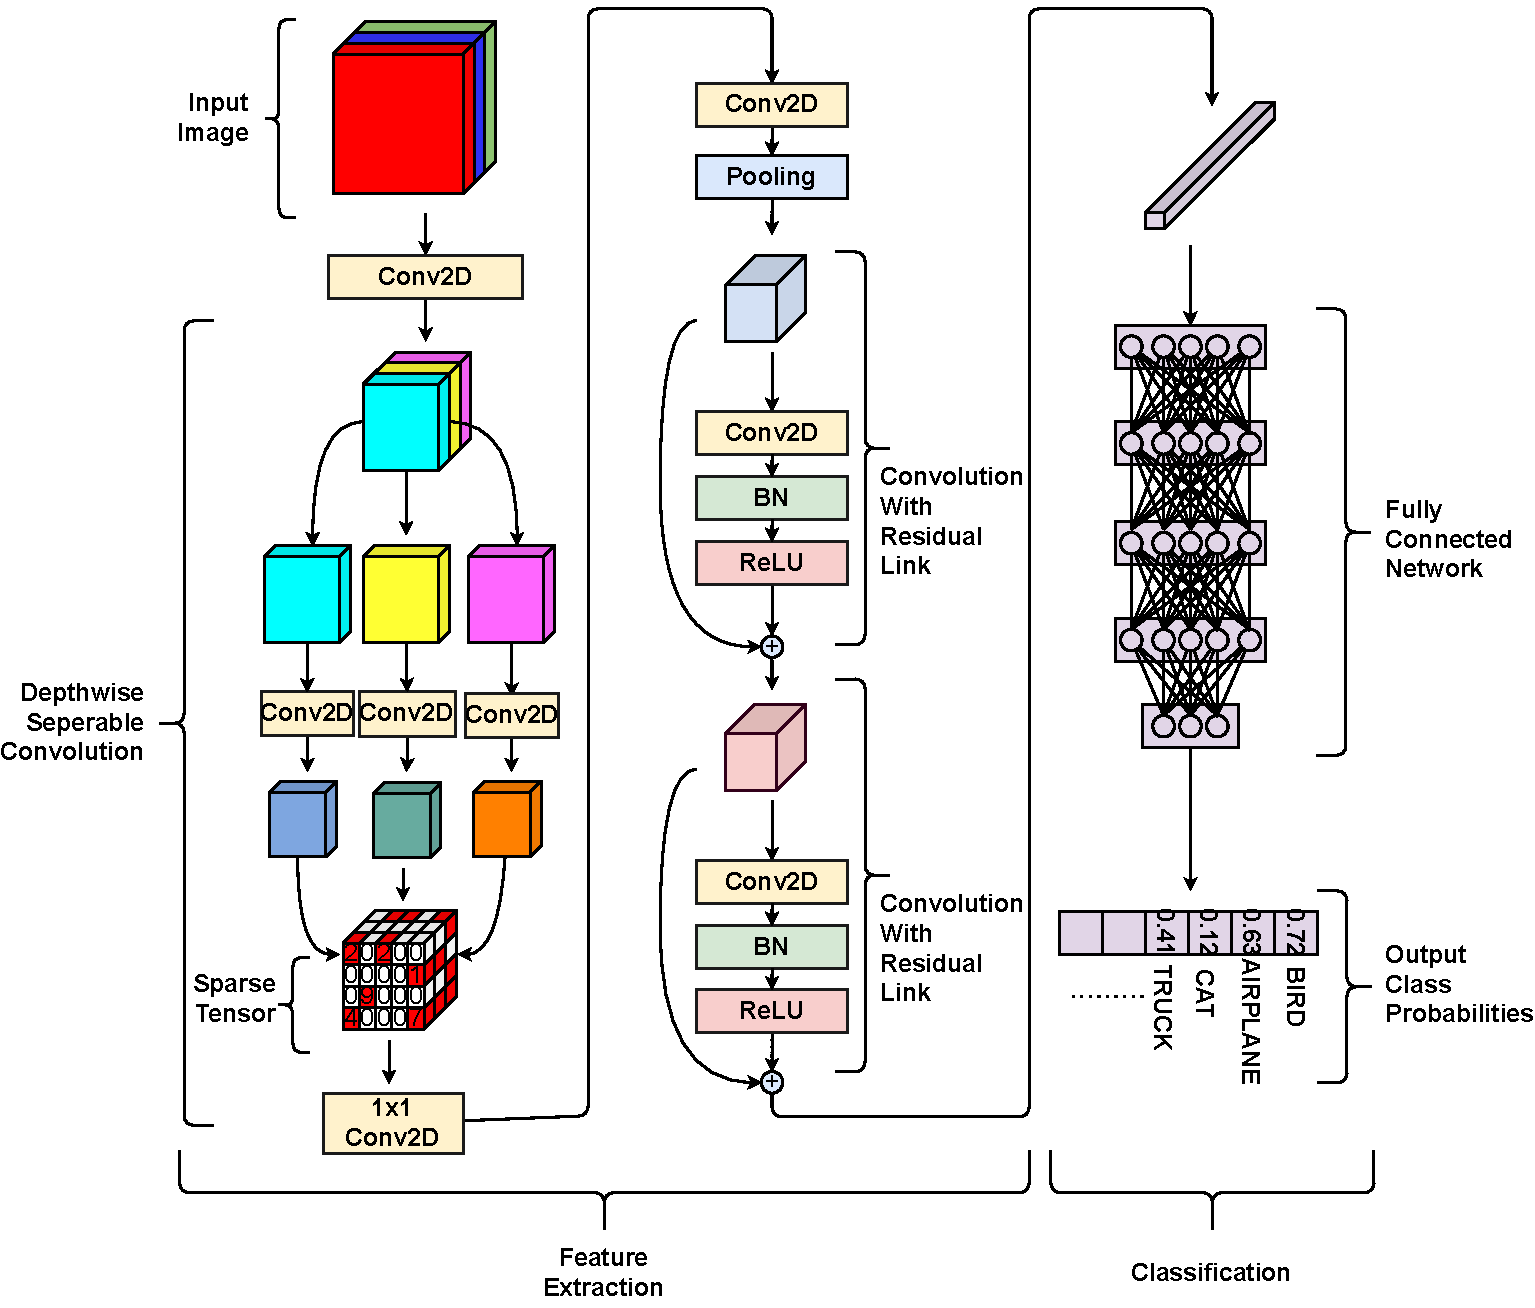
\includegraphics[scale=0.4]{fig/cnn.pdf}
    \caption{Example of the different layers in a convolution neural networks}
    \label{fig:cnn_network}
\end{figure}


Assuming the input feature map, output feature map and weight dimensionalities
of a layer are defined in \autoref{math:default_tensor_def}. A mathematical
representation of the convolution is given in \autoref{math:conv_equation_1fp}.
\autoref{math:conv_equation_1fp} represents a stencil based operation were a
sliding window called a kernel is moved across an input feature and at each
position a multiply and accumulate operation is performed to compute an output
element of the output feature map. This stencil operation is repeated for each
kernel present in the layer. The number of kernels in a layer is called the
number of filters. This multiply and accumulate operate occurs across the all
three dimensions of the IFmap tensor. In addition to the mathematical
description in \autoref{math:conv_equation_1fp} a visual representation of the
convolution operation is given in
\autoref{fig:conv_explained}.\autoref{fig:conv_explained} shows an IFmap tensor
with 3 channels (red, green, blue) being convolved with 4 separate filters each
with kernels of size 2x2. The contents of the kernels are called the weights of
the layer. Each filter's kernels operate on separate IFmap
channels. Each kernel is convolved with each IFmap channel using a sliding
window operation. The outputs across all IFmap channels are aggregated into one
OFmap channel. The total number of OFmap channels equals the total number of
Filters in the convolution layer. 

\begin{align}
    \begin{split}
        IFmap \in R^{C \times n\times n} \\
        OFmap \in  R^{F \times m\times m} \\
        Weight \in R^{F \times C\times K\times K} \\
    \end{split}
    \label{math:default_tensor_def}
\end{align}

\begin{align}
    OFmap[f][y][x] = \displaystyle\sum\limits_{c=0}^{C-1}\displaystyle\sum\limits_{k_x=0}^{K-1}\displaystyle\sum\limits_{k_y=0}^{K-1}Weight[f][c][k_y][k_x]*IFmap[c][y+ky][x+kx]
    \label{math:conv_equation_1fp}
\end{align}

\begin{figure}[ht]
    \centering
    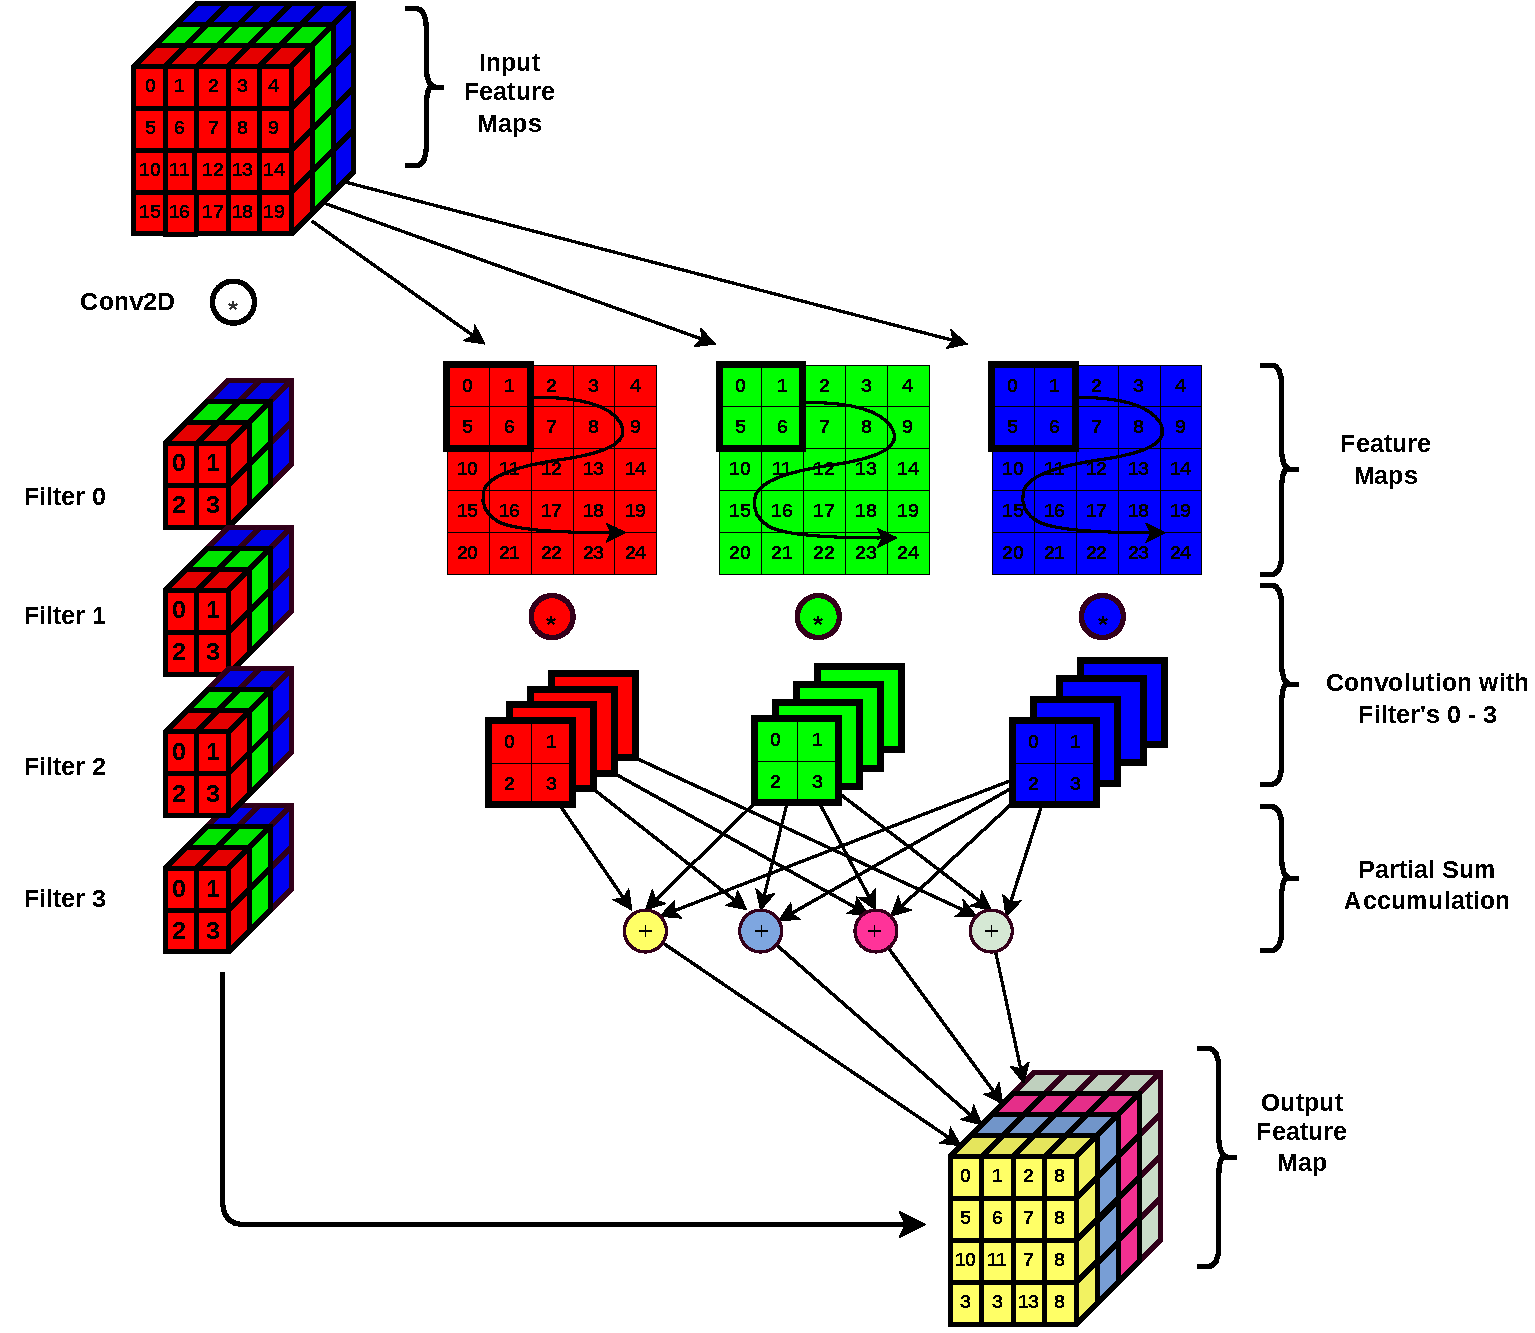
\includegraphics[scale=0.6]{fig/ConvExplained.pdf}
    \caption{Convolution Operation Illustrated}
    \label{fig:conv_explained}
\end{figure}

% \section{Computing the convolution operation}
% \label{chap:background:computing_conv}
\begin{minipage}{\linewidth}
    \begin{lstlisting}[language=C, caption=Convolution implemented as nested loops, label={lst:conv_loop}]
for(int f = 0; f < F; f++) // Filter loop
    for(int c = 0; c < C; c++) // Channel loop
        for(int y = 0; y < Y; y++) // Output feature map row
            for(int x = 0; x < X; x++)  // Output feature map col
                for(int ky = 0; ky < KY; ky++)  // Kernel row
                    for(int kx = 0; kx < KX; kx++)  // Kernel col
                        O[f][y][x] += I[c][y+ky][x+kx]*W[f][c][ky][kx];
    \end{lstlisting}
\end{minipage}

To compute the convolution operation in software we can implement the expression
in \autoref{math:conv_equation_1fp} as a series of nested for loops as in
\autoref{lst:conv_loop}. This represents a direct approach to computing
convolution layers. An alternative approach would be to converted convolution
layers to general matrix multiplication operations through several input/ output
data transformations. The advantage of reinterpreting convolutions as matrix
multiplication arises from the use highly optimized libraries for computing GEMM
like \cite{blas} on CPUs and \cite{cuBLAS} on CUDA compliant GPUs. The next
section will provide a brief overview of some of the data transformation
operations required to convert convolution into GEMM. HERO makes extensive use
of these transformations to expand it's support for a wide variety of
convolution operations outside of the common case of convolutions in the
literature. 

% However, this may not be an efficient way to compute
% convolutions given the irregular access patterns inferred by the nested loops.
% Irregular access patters may result in reduced performance due to inefficiencies
% in a processors memory hierarchy. To mitigate this irregularity a transformation
% can be applied to the inputs and outputs of a convolution layer to convert the
% overall operation into a general matrix multiplication which has a more regular
% access pattern. 

\clearpage
    
\section{Reinterpreting Convolutions As GEMM}

In the literature
\cite{cafe_con_troll} there
are several techniques used to to transform convolution operations into GEMM
using data transformations applied to the IFmaps and OFmaps of a convolution layer.
Table \ref{Table:lowering_lifting_breakdown} shows the different costs, in
floating point operations (FLOPs) and memory overhead, of the different
transformation techniques discussed in \cite{cafe_con_troll}. 

\begin{table}[!ht]
    \begin{tabular}{ll|l|l|l|}
    \cline{3-5}                                                                                                &                     & \begin{tabular}[c]{@{}l@{}}Expensive \\ Lowering/ Lifting\end{tabular}   & \begin{tabular}[c]{@{}l@{}}Balanced \\ Lowering \\ and Lifting\end{tabular} & \begin{tabular}[c]{@{}l@{}}Lowering/ \\ Expensive Lifting\end{tabular} \\ \hline
\multicolumn{1}{|l|}{\multirow{2}{*}{Lowering}}                                                   & Lowered IFmap Size   & ($k^2$C, $m^2$)                                                              & (kC, mn)                                                                    & (C, $n^2$)                                              \\ \cline{2-5} 
    \multicolumn{1}{|l|}{}                                                                            & Lowered Kernel Size & (F, $k^2$C)                                                              & (Fk, kC)                                                                    & (F$k^2$, C)                                             \\ \hline
\multicolumn{1}{|l|}{\multirow{3}{*}{\begin{tabular}[c]{@{}l@{}}Matrix \\ Multiply\end{tabular}}} & Input Size          & (F, $k^2$C)x($k^2$C, $m^2$) & (Fk, kC)x(kC, mn)                              & (F$k^2$, C)x(C, $n^2$)                   \\ \cline{2-5} 
    \multicolumn{1}{|l|}{}                                                                            & \# FLOPS            & 2F$k^2$C$m^2$                                                            & 2F$k^2$Cmn                                                   & 2F$k^2$C$n^2$                            \\ \cline{2-5} 
    \multicolumn{1}{|l|}{}                                                                            & Output Size         & (F, $m^2$)                                                               & (Fk, mn)                                                                    & (F$k^2$, $n^2$)                          \\ \hline
    \multicolumn{1}{|l|}{\multirow{2}{*}{Lifting}}                                                    & \# FLOPS            & 0                                                                        & $m^2$kF                                                      & $m^2$$k^2$F                              \\ \cline{2-5} 
    \multicolumn{1}{|l|}{}                                                                            & \# Ram Read         & F$m^2$                                                                   & Fkmn                                                                        & F$k^2$$n^2$                              \\ \hline
    \end{tabular}
\label{Table:lowering_lifting_breakdown}
    \caption{Breakdown of the dimensionalities and complexity (in FLOPs and Ram Reads) of the different available lowering and lifting strategies adapted from \cite{cafe_con_troll}}
\end{table}

The first of the transformation techniques used in computing convolution
operations as general matrix multiplication discussed in \cite{cafe_con_troll}
is the Im2Col transformation or as \cite{cafe_con_troll} refers to it
"Expensive lowering/lifting". The lowering/ lifting nomenclature arises from
reduction of the IFmap and Weight tensor dimensionalities from 3D to 2D and vice
versa for the OFmap. The expensive descriptor arises from the substantial
increase in memory allocation required from lowering the IFmap input into two
dimensions as a result of data duplication. 

Expensive lowering and lifting "flattens" the IFmap by positioning a
hypothetical stencil where the real stencil would be positioned in the
convolution operation and collects all the IFmap elements present in that
stencil into one row of an IFmap matrix. The stencil's dimensions are proportional to
the kernel size in the weight tensor. This collection processes is repeated
for every real stencil position present in the original convolution operation.
The stencil is moved through the IFmap tensor following a sliding window pattern.
Since stencil positions are usually very close to each other (depending on the
stride size of the layer) a substantial amount of IFmap elements are reused
between stencil positions. The act of lowering the contents of each stencil
position into one row results in the duplication of IFmap elements between
consecutive rows in the IFmap matrix.  
The weight kernels for each filter are flattened vertically into a weight
matrix. The OFmap matrix is then produced by matrix multiplication between the
IFmap and weight matrices. To recover the OFmap tensor a "lifting" operation is
performed by reshaping the output OFmap matrix into a 3D tensor. An illustration
for expensive lowering/ lifting is given in \autoref{fig:im2col}. In
\autoref{fig:im2col} a 4x4x3 IFmap is lowered into a matrix using expensive
lowering. Each row of the matrix represents the contents of a single stencil
position. The weight tensor of size 2x2x3x4 is also lowered into a matrix. Each
filter in the weight tensor is transformed into a column in the weight matrix.
The multiplication of both of the IFmap and weight matrices produces the OFmap
matrix. The lifting operation performed on the OFmap matrix reshapes the matrix
into a 3D tensor by converting each column of the OFmap matrix into a channel in
the OFmap tensor. 

\begin{figure}[!ht]
    \centering
    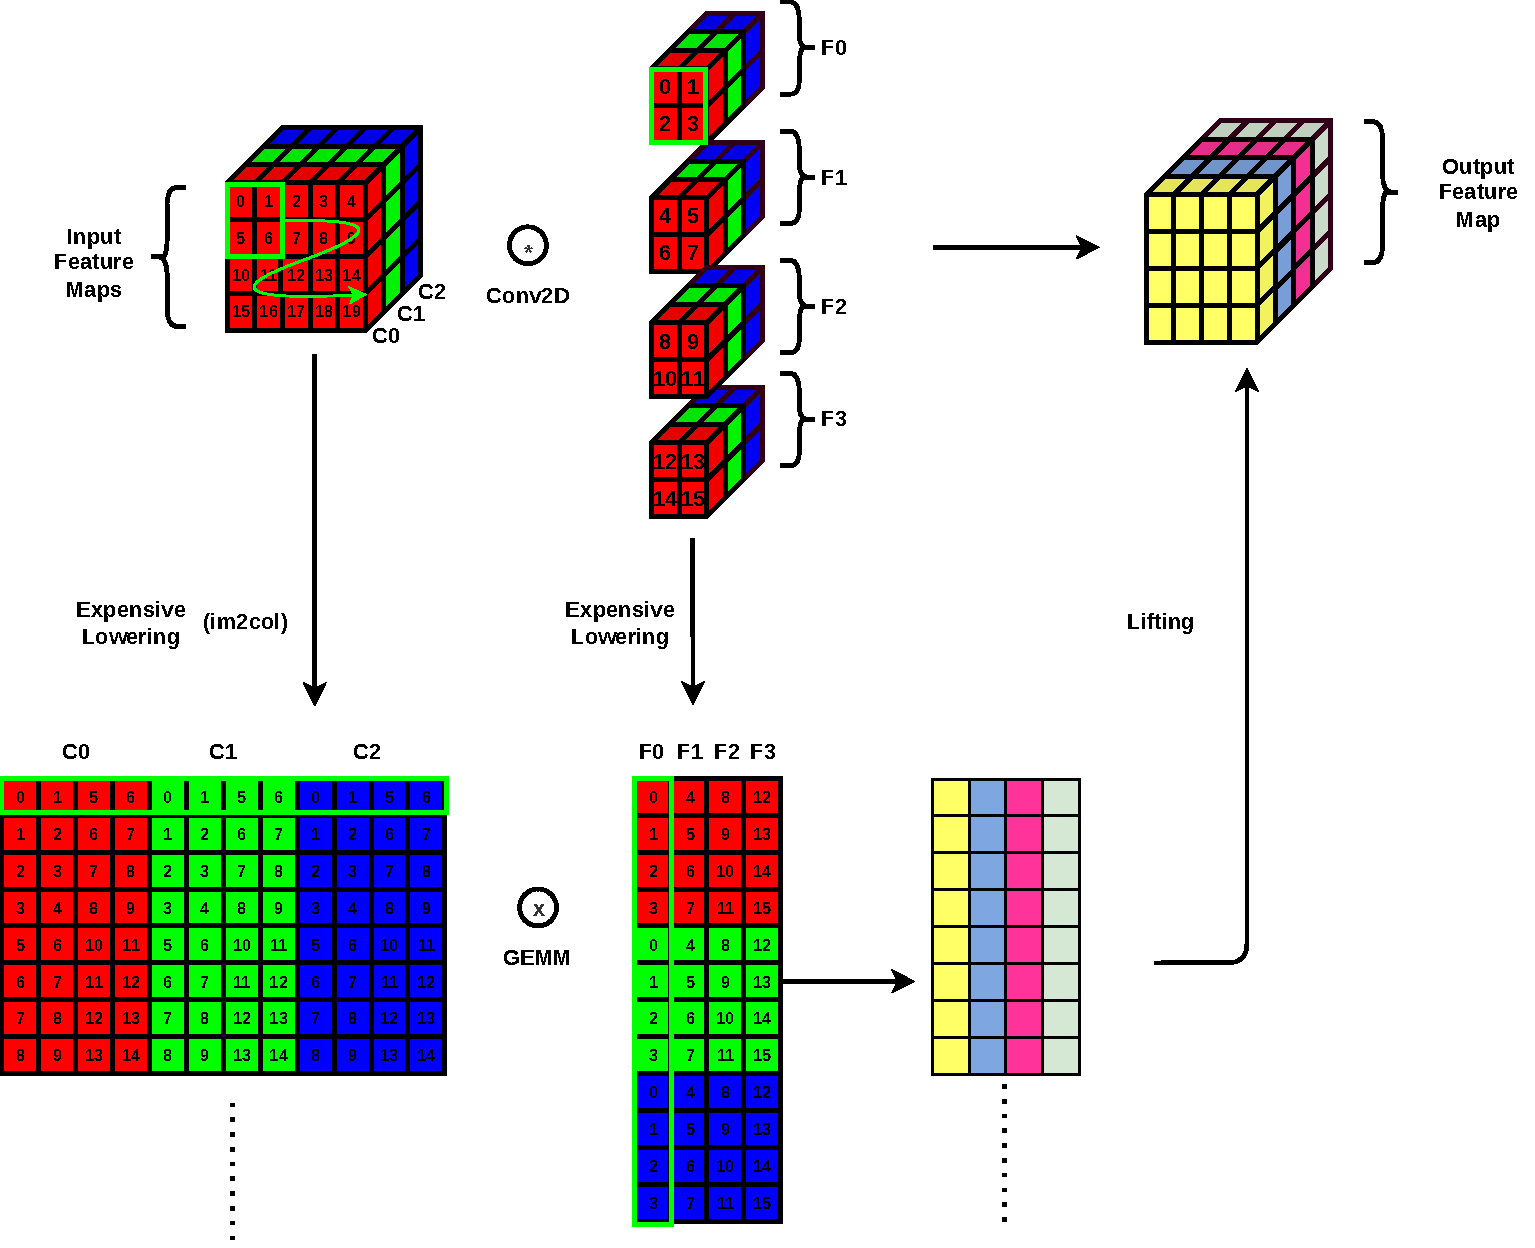
\includegraphics[scale=0.6]{fig/Im2Col.pdf}
    \caption{Im2Col (Expensive lowering/ lifting) Illustrated}
    \label{fig:im2col}
\end{figure}

An alternative approach to expensive lowering/ lifting is balanced lowering and
lifting. Analytical expressions that describe balanced lowering/ lifting adapted
from \cite{cafe_con_troll} are given in \eqref{math:balanced_lowering_ifmap} -
\eqref{math:balanced_lifting_ofmap} with the inclusion of lowering in the
presence of multiple filters to describe these data transformation operations.
In addition, to supplement the analytical expressions balanced lowering
presented \autoref{fig:balanced_lowering_lifting} is used to clarify the
available expressions further.  

In balanced lowering, we first lower the ifmap and weights using expression
\eqref{math:balanced_lowering_ifmap} and \eqref{math:balanced_lowering_weight}.
Then a matrix multiplication is performed in \eqref{math:balanced_lowering_gemm}
followed by a lifting operation. Unlike the lifting operation in the expensive
lowering/ lifting transformation, lifting in the balanced transformation
involves a series vector operation in addition to a reshape of the output OFmap
matrix. Balanced lowering has the advantage of reduced data duplication in the
IFmap and trades that off with increasing the number of FLOPs for lifting the
OFmap. \autoref{fig:balanced_lowering_lifting} illustrates balanced lowering/
lifting on a 5x5x3 IFmap and a 2x2x3x4 weight tensor. The same stencil based
intuitive explanation presented for expensive lowering/ lifting applies here
with a few modification. For IFmap lowering, instead of using a full sized 2x2
stencil to collect the IFmap tensor contents a half sized 1x2 stencil is used.
The stencil dimensions remain proportional to the weight tensor's kernel size.
The sliding window pattern still applies when moving the stencil through the
IFmap. However, instead of moving the stencil horizontally through IFmap then
vertically we first move the stencil vertically then horizontally through the
IFmap tensor. Each position of the stencil corresponds to one output row in the
IFmap matrix. Lowering the weight tensor is similar to expensive lowering in
that the contents of each filter are lowered into columns of the weight matrix.
However, instead of each filter occupying 1 column of the weight matrix, each
filter row and it's associated channels occupies 1 column in the weight matrix.  
 
\begin{align}
    \begin{gathered}
        IFmap \in R^{C\times n\times n} \xrightarrow[]{Balanced Lowering} \hat{IFmap} \in R^{nm\times KC} \\
        \hat{IFmap}[cn+r, :] = vec(IFmap[:, r, c:c+K]) \\
        \forall r,c \in [0, n-1], [0, m-1]
    \end{gathered}
    \label{math:balanced_lowering_ifmap}
\end{align}

\begin{align}
    \begin{gathered}
        Weight \in R^{F\times C\times K \times K} \xrightarrow[]{Balanced Lowering} \hat{Weight} \in R^{KC\times FK}\\
        \hat{Weight}[f*K:f*K+K, i] = vec(Weight[f, :, i, :]) \\
        \forall f,i \in [0, F-1], [0, K-1]
    \end{gathered}
    \label{math:balanced_lowering_weight}
\end{align}

\begin{align}
    \begin{gathered}
        \hat{OFmap} = \hat{IFmap}.\hat{Weight}
    \end{gathered}
    \label{math:balanced_lowering_gemm}
\end{align}

\begin{align}
    \begin{gathered}
        \hat{OFmap} \in R^{nm\times FK} \xrightarrow[]{Balanced Lifting} OFmap \in  R^{m\times m\times F}\\
        OFmap[f, r, c] = (\displaystyle\sum\limits_{j=0}^{K-1} \hat{OFmap}[cn+r+j, j+fK]) \\
        \forall f,r,c \in [0, F-1], [0, m-1], [0, m-1]
    \end{gathered}
    \label{math:balanced_lifting_ofmap}
\end{align}

\begin{figure}[!ht]
    \centering
    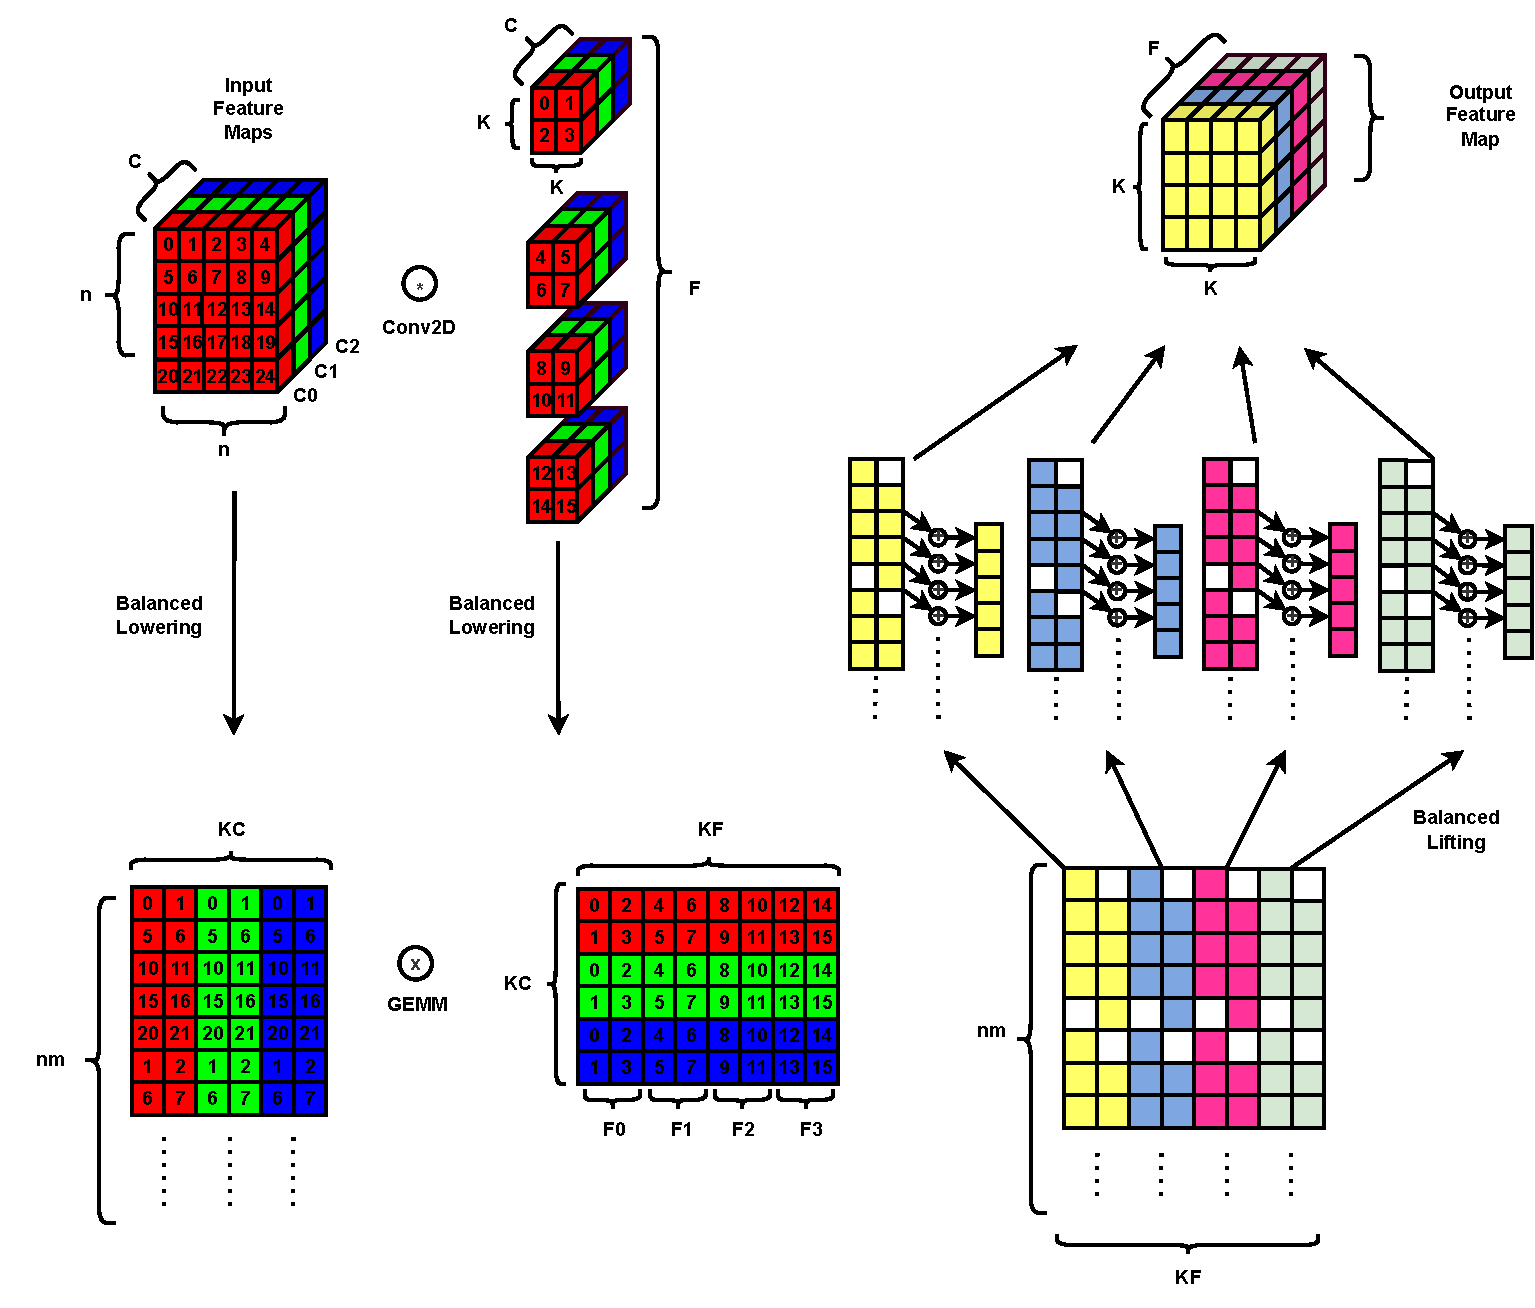
\includegraphics[scale=0.6]{fig/BalancedLoweringLifting.pdf}
    \caption{Balanced Lowering/Lifting Illustrated}
    \label{fig:balanced_lowering_lifting}
\end{figure}

The third (lowering/ expensive lifting) strategy further trades off the
the size of the lowered matrices by increasing the complexity of lifting.
However, this strategy diminished the gains from converting convolution layers
to general matrix multiplication and therefore are not elaborated on in this
thesis. \autoref{Table:lowering_lifting_breakdown} breakdown the
dimensionalities and complexities of the three strategies discussed in
\cite{cafe_con_troll} using the dimensions of the IFmap, OFmap, and Weight
tensors defined in \autoref{math:default_tensor_def}.

HERO takes advantage of the aforementioned data transformation approaches to
convert unsupported convolution operations into GEMM operations. However, HERO
is optimized for the common case of convolutions which allows it to run a subset
of the convolution operations in the literature directly. HERO implements this
subset of convolution operations as dataflow operations in hardware. As
mentioned in the introduction of this chapter in order to explore the
accelerator dataflow design space available to HERO we must first define the
dataflow design space. This will be the focus of the next section.  

    
\section{Implementing convolutions in hardware}
\subsection{The dataflow taxonomy}


From \cite{dnn_df_overrated} 
dataflows can be defined using the direct convolution
nested loop structure combined with unroll pragmas. Listing
listing \ref{lst:conv_loop_with_pragmas} expands on listing \ref{lst:conv_loop}
by including unroll pragmas on all of the for loops. What defines that dataflow is 1) loop unroll
targets (which loops are unrolled) 2) loop order 3) the unroll factors of the
unrolled loops. These choices influence the stationarity of different data
elements used in the convolution operation. 


\begin{minipage}{\linewidth}
    \begin{lstlisting}[language=C, caption=Convolution implemented as nested loops, label={lst:conv_loop_with_pragmas}]
#pragma UNROLL F_T
for(int f = 0; f < F; f+=F_T) // Filter loop
#pragma UNROLL C_T
    for(int c = 0; c < C; c+=C_T) // Channel loop
#pragma UNROLL Y_T
        for(int y = 0; y < Y; y+=Y_T) // Output feature map row
#pragma UNROLL X_T
            for(int x = 0; x < X; x+=X_T)  // Output feature map col
#pragma UNROLL KY_T
                for(int ky = 0; ky < KY; ky+=KY_T)  // Kernel row
#pragma UNROLL KX_T
                    for(int kx = 0; kx < KX; kx+=KX_T)  // Kernel col
                        O[f][y][x] += I[c][y+ky][x+kx]*W[f][c][ky][kx];
    \end{lstlisting}
\end{minipage}

Listing \ref{lst:conv_loop_ws} shows a generic
implementation of a single convolution layer with all layers unrolled except the
output feature map loops. The pragmas define the unroll
targets and the constants in the pragmas define the unroll factors. 
Weight elements within a
kernel remain stationary throughout the computation of an output feature map
until a new tile of channels C\_T is loaded into the accelerator. Once the
weights within a particular channel and filter group are used to produce an
output feature map they are discarded and are only loaded again when computing
the same layer for a new input image. The choice of loop unroll targets, factors
and loop ordering in listing \ref{lst:conv_loop_ws} creates a common dataflow in
the literature called weight stationary.

\begin{minipage}{\linewidth}
    \begin{lstlisting}[language=C, caption=Convolution implemented as nested loops, label={lst:conv_loop_ws}]
#pragma UNROLL F_T
for(int f = 0; f < F; f+=F_T) // Filter loop
#pragma UNROLL C_T
    for(int c = 0; c < C; c+=C_T) // Channel loop
        for(int y = 0; y < Y; y+=Y_T) // Output feature map row
            for(int x = 0; x < X; x+=X_T)  // Output feature map col
#pragma UNROLL KY_T
                for(int ky = 0; ky < KY; ky+=KY_T)  // Kernel row
#pragma UNROLL KX_T
                    for(int kx = 0; kx < KX; kx+=KX_T)  // Kernel col
                        O[f][y][x] += I[c][y+ky][x+kx]*W[f][c][ky][kx];
    \end{lstlisting}
\end{minipage}
 

From listing \ref{lst:conv_loop_ws} we
can see that from the loop unroll targets and loop unroll factors there are many
other possible dataflow configurations available to us outside of weight
stationary. Additionally, since accelerators are generally limited to two
spatial axis the loops of the convolution operation can be mapped to two spatial
axis. If we allow multiple convolution loops under some kernel unroll factor
KY\_T/KX\_T  to be unrolled and mapped to the same accelerator spatial axis we
can influence the effective unroll factors when performing different
convolutions of different kernel sizes other than KY\_T/KX\_T. The choice of
which loops are mapped to which spatial axis is an additional design dimension
alongside loop unrolling. 

With the dataflow design space defined by \cite{dnn_df_overrated} a data driven
exploration of the dataflow design space becomes possible. Combining network
configuration data provided by CIGAR with  \cite{dnn_df_overrated} dataflow
taxonomy will enables us to define HERO's dataflow for the common case of
convolutions in the literature. However, a dataflow choice needs to be matched
with an appropriate hardware implementation. In the next section an accelerator
hardware implementation taxonomy is introduced from \cite{maestro}. The
available hardware implementation options in the taxonomy are determined by
communication and reuse behavior of the different data elements in a chosen
dataflow. The hardware taxonomy presented in the next section will be used in
tandem with the dataflow taxonomy to define HERO's implementation in hardware.  

\subsection{The Hardware Implementation taxonomy}

\begin{figure}
    \centering
    \subfigure[]{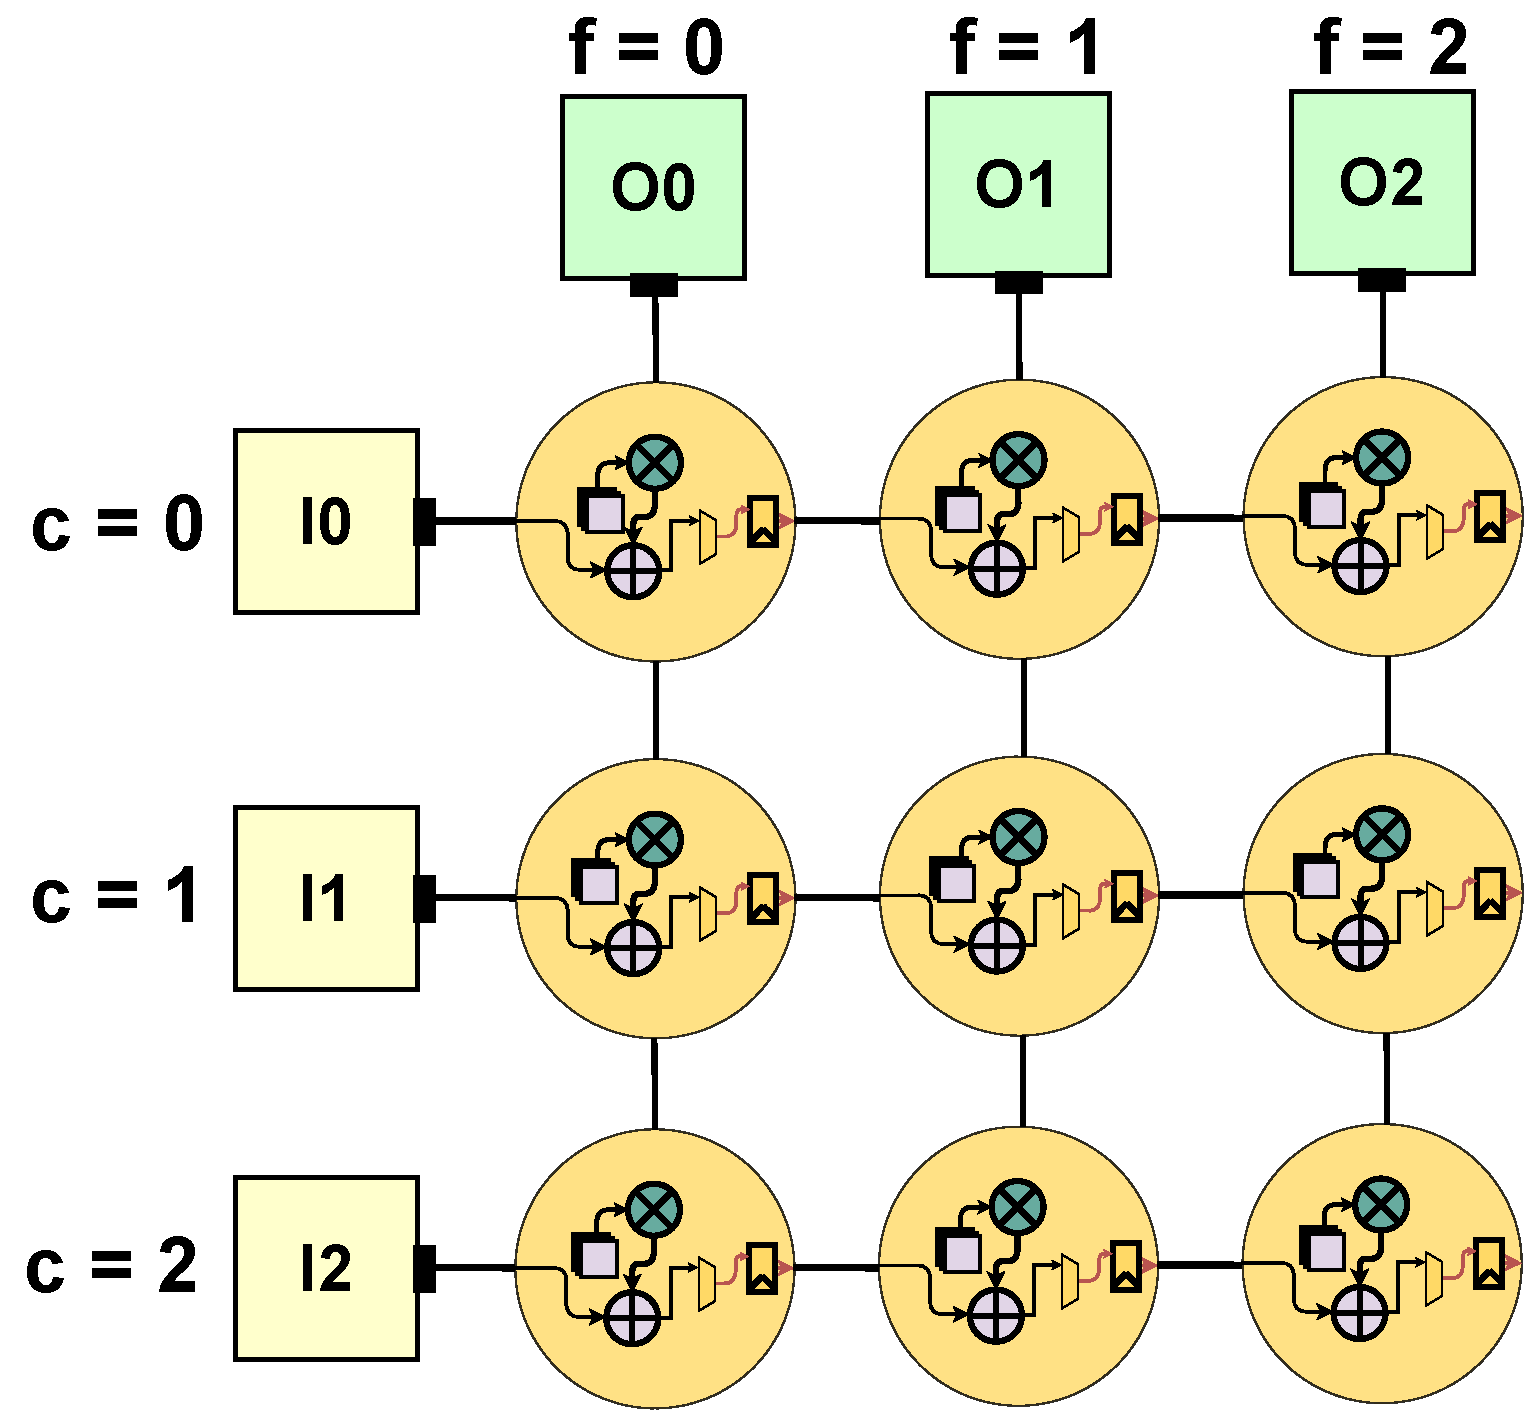
\includegraphics[width=0.32\textwidth]{fig/unroll_c_f.pdf}}
    \hspace{0.1cm} 
    \subfigure[]{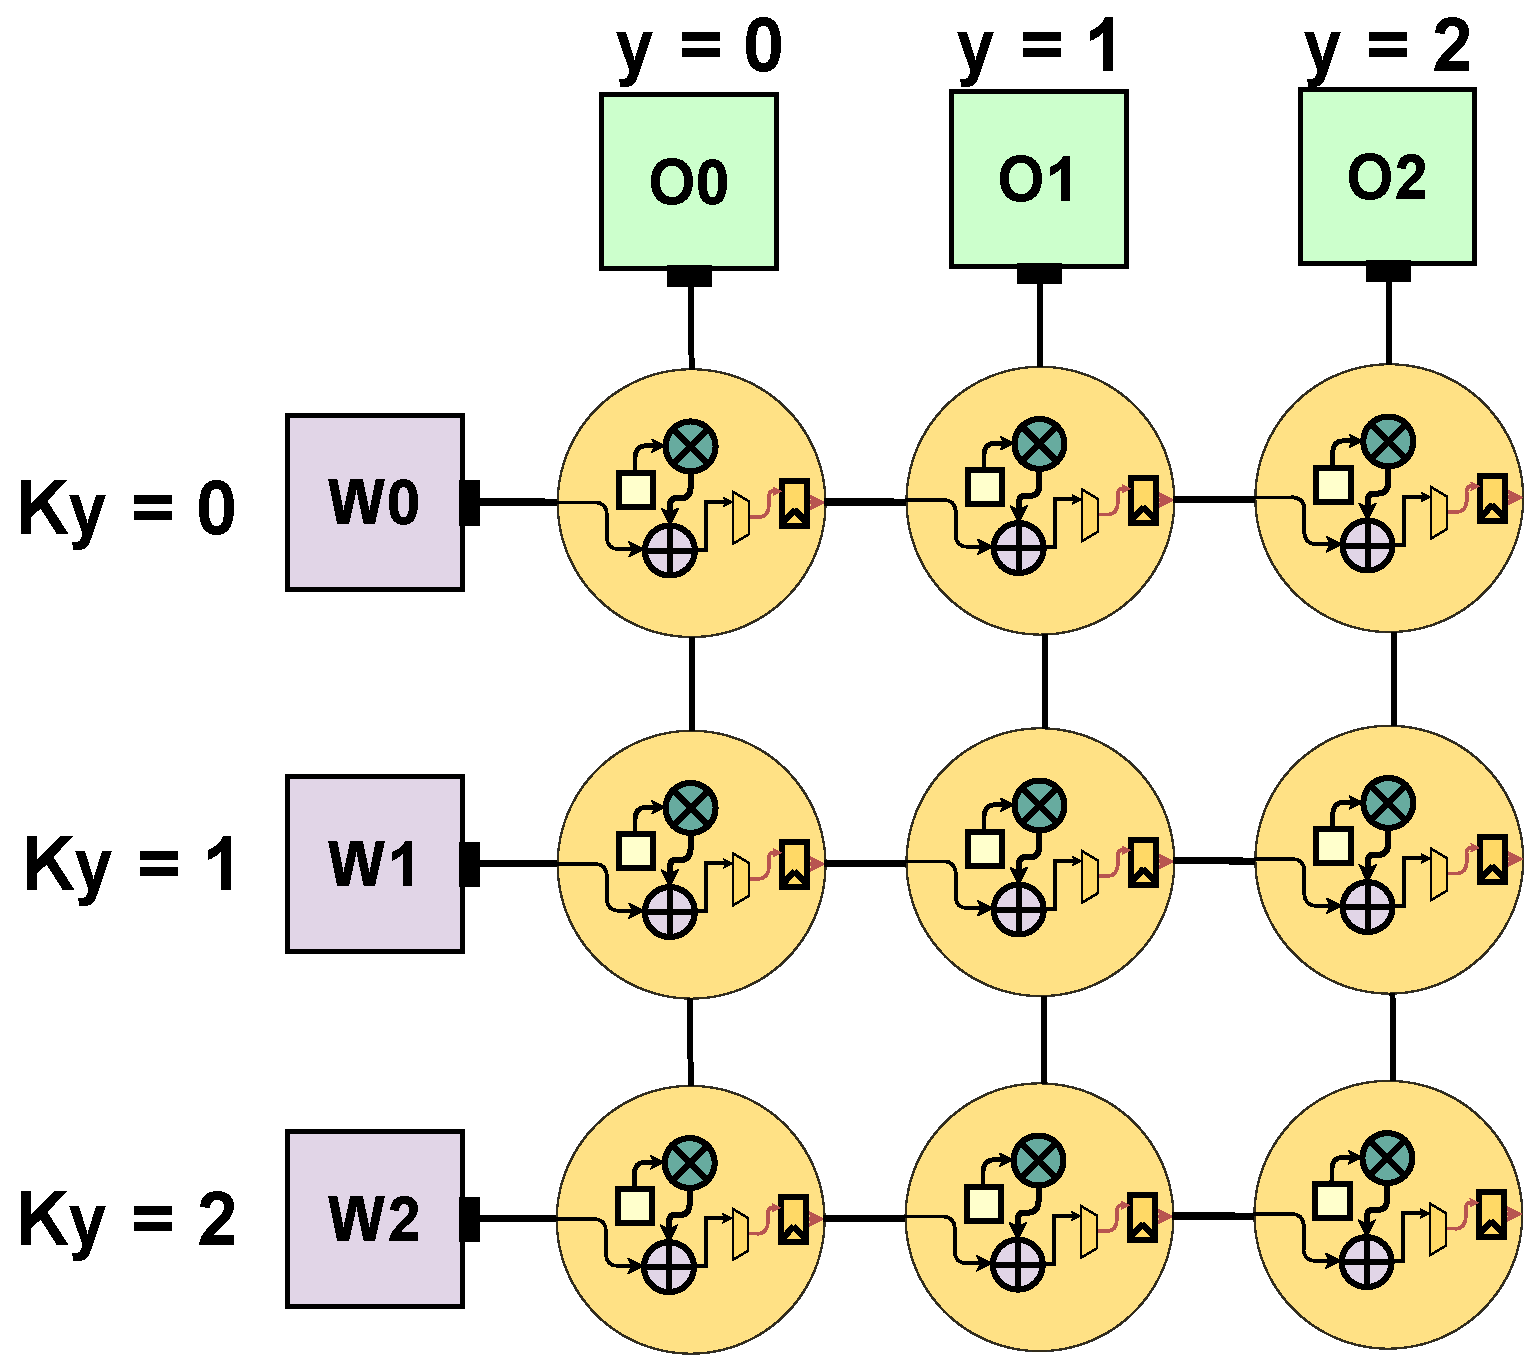
\includegraphics[width=0.32\textwidth]{fig/unroll_fy_y.pdf}}
    \hspace{0.1cm} 
    \subfigure[]{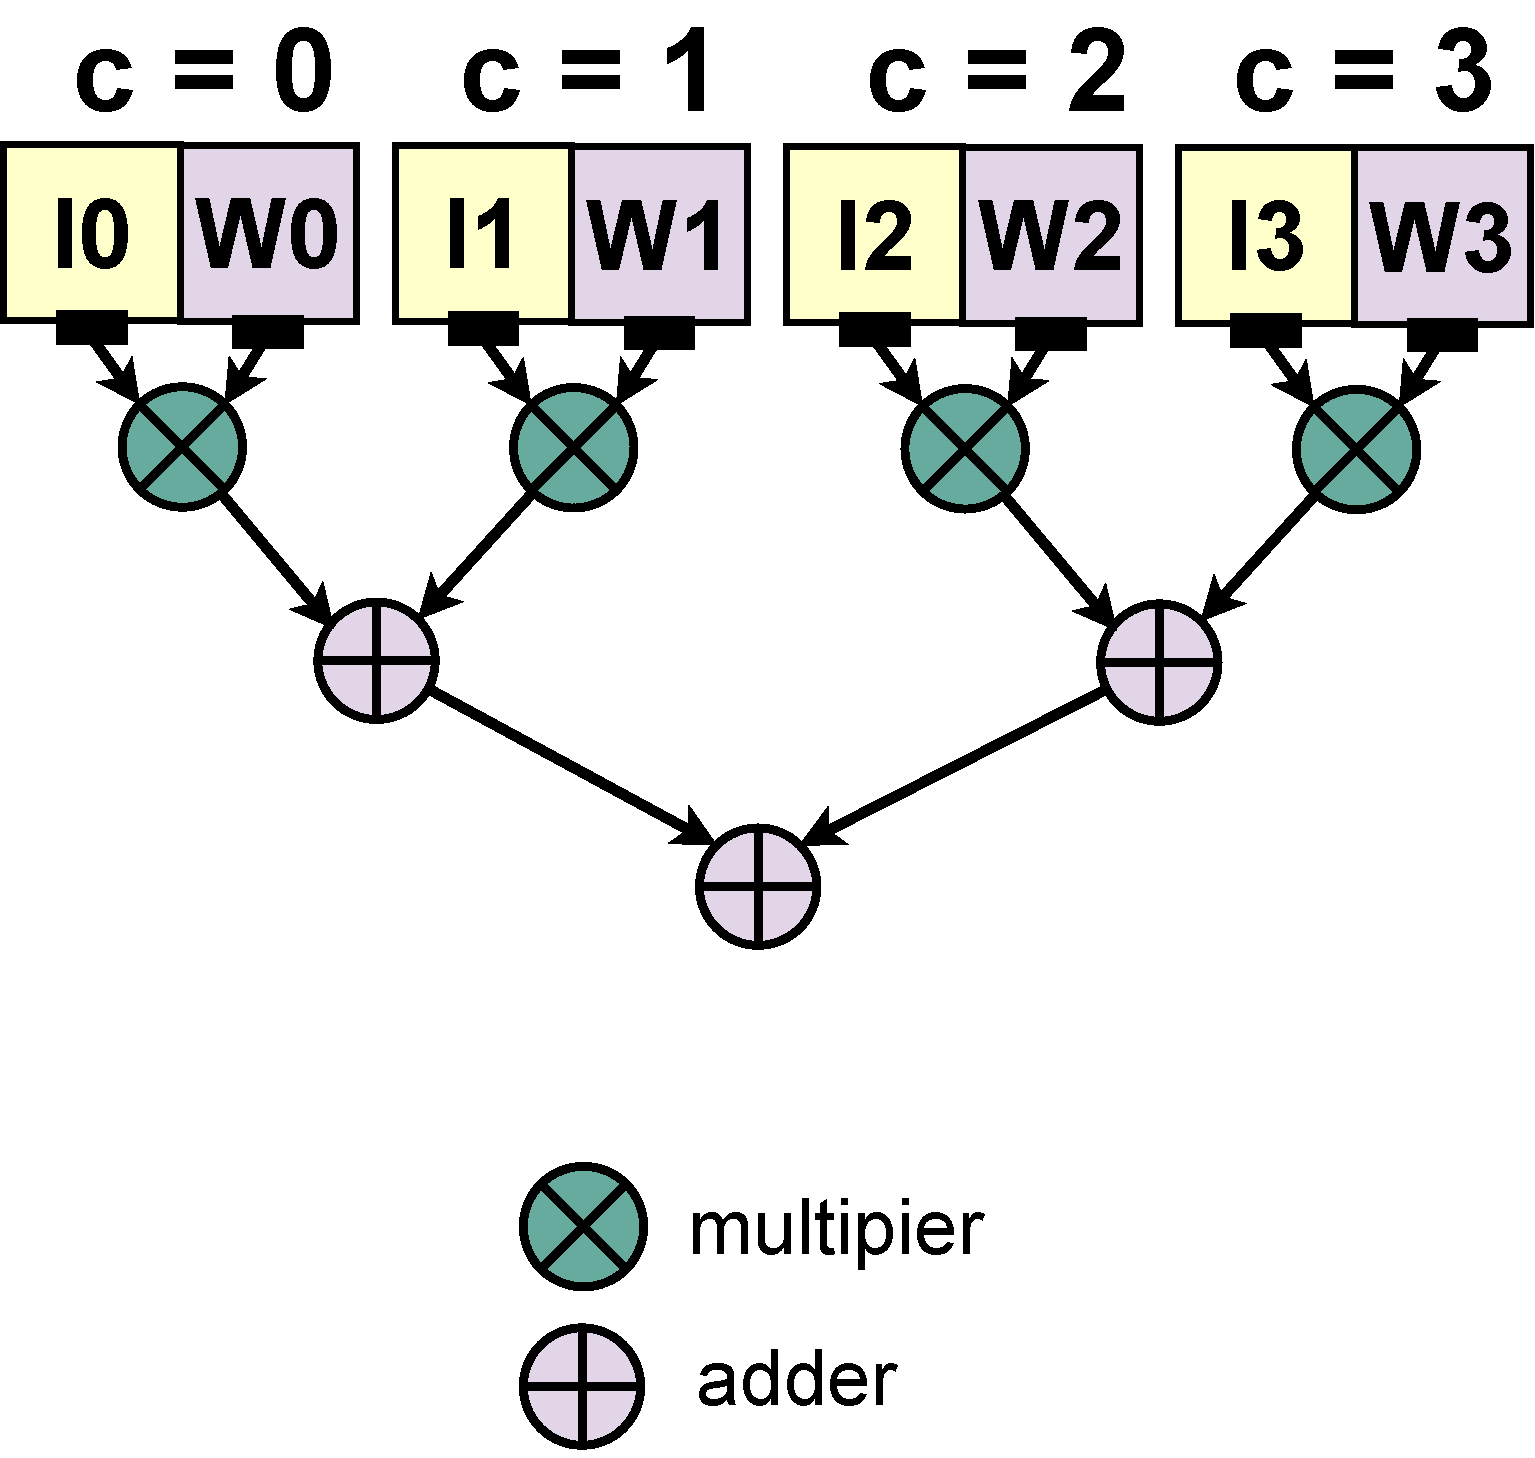
\includegraphics[width=0.32\textwidth]{fig/unroll_c.pdf}} 
    \hspace{0.1cm} 
    \subfigure[]{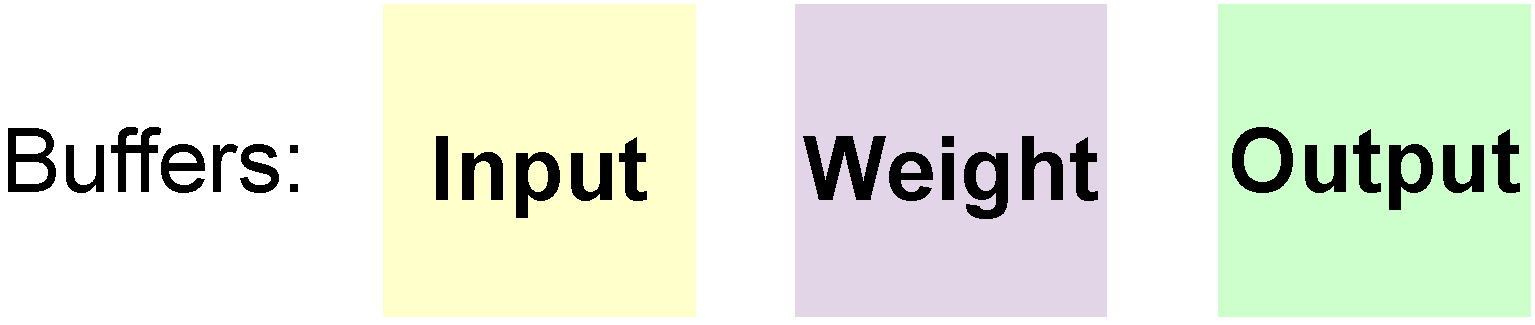
\includegraphics[width=0.3\textwidth]{fig/buffer_description.pdf}}
    \caption{Illustration of different dataflow implementations (adapted
    from\cite{dnn_df_overrated}) arising from (a) Unrolling F and C loops (b)
    unrolling Ky and Y loops (c) unrolling C loops}
    \label{fig:unroll_illustration}
\end{figure}

\begin{figure}[ht]
    \centering
    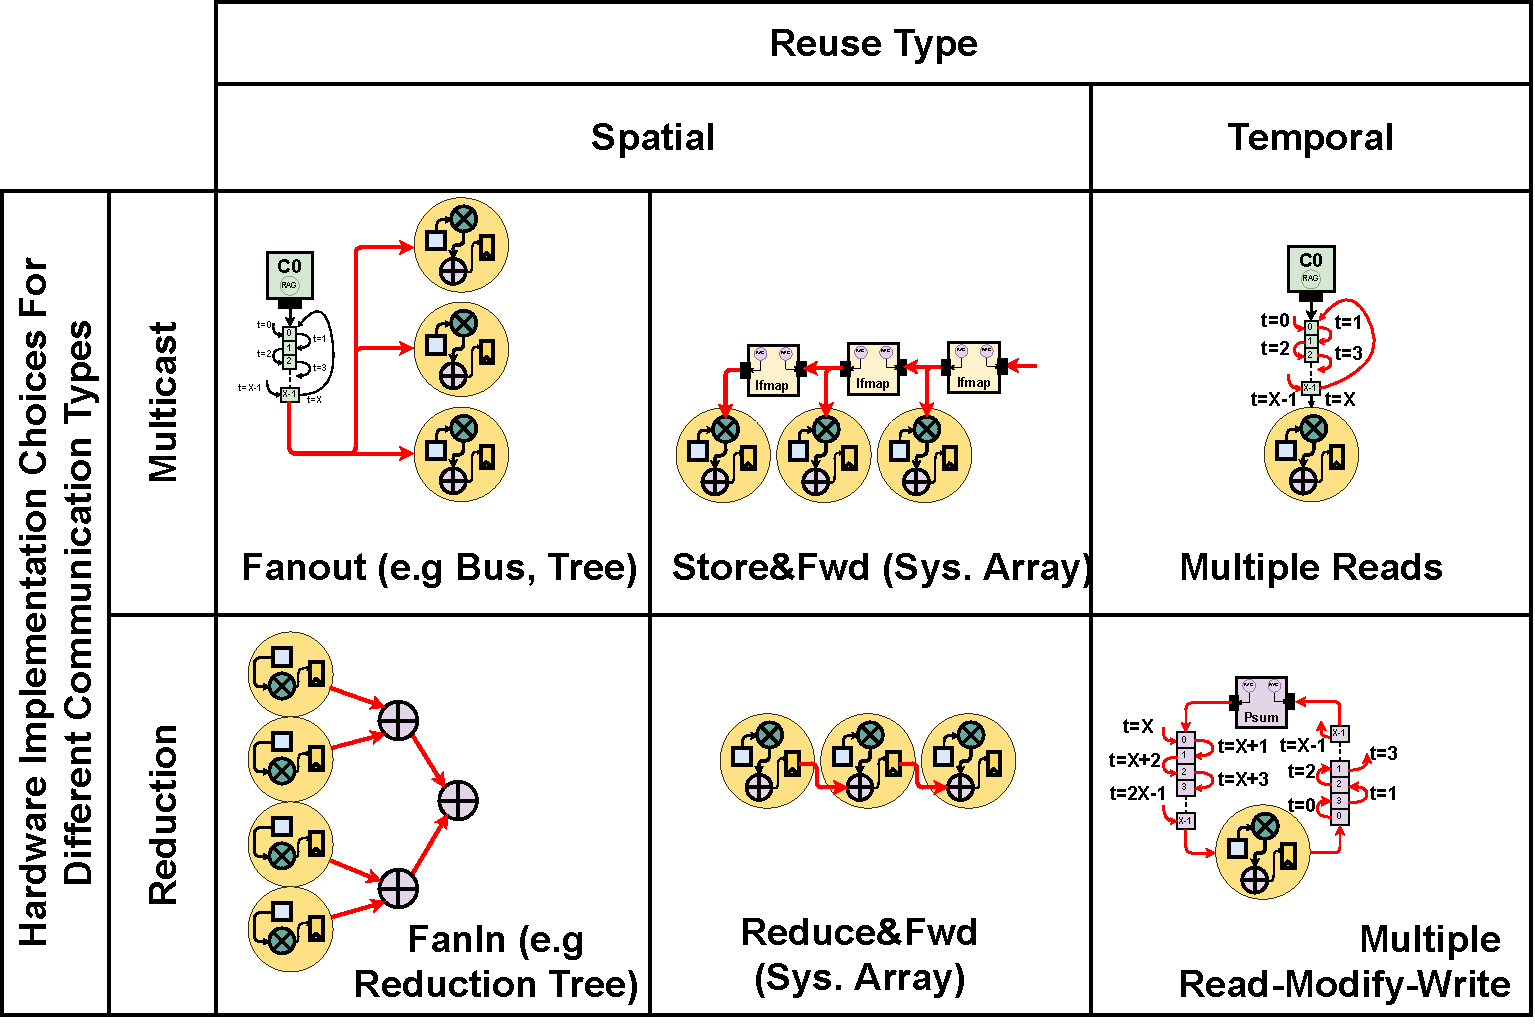
\includegraphics[scale=0.58]{fig/hw_taxonomy.pdf}
    \caption{Hardware Implementation Taxonomy adapted from \cite{maestro}}
    \label{fig:hw_taxonomy}
\end{figure}


Depending on the dataflow selected using the dataflow taxonomy (1) loop ordering
(2) unroll targets (2) loop unroll factors. The implementation options are
derived based on the type of reuse present in the dataflow. Following the
hardware implementation taxonomy presented in in \cite{maestro}, we can classify
the available hardware implementation options based on the the type of reuse is
spatial where a data element is read and used in the same cycle or temporal
where a data element is read in one cycle and reused after several cycles.
Depending on the nature of the reuse, if it is read or read modify write, there
are several options for supporting the communication inferred from that reuse
type. To deduce the type of reuse and overall communication behavior for each
data element in any dataflow we can use the polyhedral model to detect temporal
reuse. Spatial reuse detection can be inferred directly from the loops. The
application of the polyhedral to infer temporal reuse behavior as well as the
inference of spatial reuse directly from the convolution loops is discussed in
\autoref{chap:dda}.

Figures in \autoref{fig:unroll_illustration} show different reduction/ multicast
schemes based on reuse behavior of data elements (IFmap, OFmap, Weights)
apparent in the dataflow. The space of available schemes is not limited to those
presented in \autoref{fig:unroll_illustration} though. The full hardware
taxonomy from \cite{maestro} is illustrated in figure \autoref{fig:hw_taxonomy}.
The hardware taxonomy presented in this section will be used in tandem with the
dataflow taxonomy to define HERO's implementation in hardware. Note that the
usage of this taxonomy will span both operational modes of HERO, direct
convolution acceleration as well GEMM. What enables this taxonomy to be applied
to GEMM is the overlap between GEMM and the depthwise convolution operation. A
discussion of how these two operations overlap is presented in
\autoref{chap:dda:dataflow_dse:GEMM_mode}. 


\section{Related work}
\label{chap:related_work}

To contrast this work with other works in the literature a brief discussion of
competing accelerator designs is presented in this section. Note that the
related works discussion is limited to competing accelerator designs meant for
ASIC based implementations. Convolution accelerator generators targeting FPGAs
are not discussed here.

\subsection{Eyeriss V1 and V2}
\label{chap:related_work:eyeriss}

Eyeriss \cite{isscc_2016_chen_eyeriss} is an accelerator for state-of-the-art
deep convolutional neural networks (CNNs). It attempts to optimize for the
energy efficiency of the entire system by minimizing data movement between the
accelerator and DRAM thus reducing data movement energy. Eyeriss achieves these
goals by using a the row stationary (RS) dataflow on a spatial architecture with
168 processing elements. 

EyerissV2 \cite{eyerissv2} improve on EyerissV1 by proposing an architecture
optimized for sparse and compact DNNs. To account for the substantial variation
between different CNN layer it introduces a highly flexible on-chip network,
called hierarchical mesh, that can adapt to the different amounts of data reuse
and bandwidth requirements of different data types. THe goal of the mesh is to
improve the utilization of the computation resources.

EyerissV1 and EyerissV2 do not optimize for linear layers. Linear layers may not
represent a substantial portion of a CNN network runtime, however, some models
use linear layers exclusively. These models are underrepresented in vision based
tasks however, they are present in NLP based tasks. An examples of these
models includes the Transformer model \cite{transformer_model}. This limits how general the
Eyeriss architecture is when used for models outside of the vision domain. This
work aims to build an accelerator that accounts for the importance of linear
layers in those models. 

\subsection{Tensor processing unit}
\label{chap:related_work:tpu}

At the heart of a TPU is a 65,536 8-bit MAC matrix multiply unit that offers a
peak throughput of 92 TeraOps/second (TOPS) and a large (28 MiB)
software-managed on-chip memory \cite{tpu}. The TPU emphasizes efficiency in
computing matrix multiplication above all other operations. With the
aforementioned transformations used to convert convolution layers to general
matrix multiplication the TPU is able to accelerate a wide variety of
computation workloads given the generality of the operation it's hardware
accelerates. This generality comes at the cost of efficiency in computing
convolution layers given the overheads of the transformations discussed in the
prior sections. This works aims to mitigate this inefficiency while maintaining
support for a wide variety of computation workloads. 


\subsection{Maeri}
\label{chap:related_work:maeri}

Since most DNN accelerators support only fixed dataflow patterns internally
mapping arbitrary layer dataflows to these fabric efficiently is challenging.
Mapping inefficiencies can lead to under utilization of the available compute
resources. DNN accelerators need to be configurable internally to support the
various dataflow patterns that could be mapped over them. To address this
\cite{maeri} introduces MAERI, a DNN accelerator built with a set of modular and
configurable building blocks backed by a flexible on-chip network capable of
supporting a myriad of DNN partitions and mappings. 

MAERI aims to support a wide variety of DNN layers and mappings by moving the
complexity of data orchestration to runtime configuration of a flexible on-chip
NOC. The drawback of this approach is the complexity of the NOC as well as the
area it occupies on-chip. This work aims to combine the runtime flexibility of
data orchestration on-chip through the use of a novel data orchestration
primitive called self addressable memory (SAMs) discussed in
\autoref{chap:data_orchestration} with the small area footprint of a fixed
on-chip fabric optimized through a novel optimizer presented in
\autoref{chap:arch_dimensioning}. 


% \section{Analysis of data reuse with the polyhedral model}

% \cite{meeus} used polyehdral model to analyse reuse within stencil based applications described
% as nested loops. One important element in their approach is their program written in iscc that
% can determine temporal reuse of data elements

% There's the polyhedral extraction tool out there but unfortunately there's no
% way to encode parallelism or loop unrolling in it without relying on compiler
% pragmas. 

% below is an example of this reuse applied to the gemm loops
